\section{Implications for Earth's Future}\label{earth-implications}

A key insight from our modeling is that the parameters governing recovery (the recovery fraction $r_f$ and the recovery delay $r_d$) are not fixed properties of a civilization but can be deliberately engineered. Investments in civilizational continuity infrastructure directly map onto these parameters: a higher $r_f$ corresponds to greater preservation of knowledge, technology, and resources through collapse events, while a lower $r_d$ corresponds to faster institutional and technological rebuilding. Together, improvements in these parameters increase the duty cycle $D_c$ and thus, increase the fraction of time civilization remains functional and productive.

The concept of "recovery kits" (curated repositories of essential knowledge designed to accelerate post-collapse rebuilding) represents one practical approach to raising $r_f$. \citet{Dartnell2014-tk} has explored in detail the minimum knowledge base required to reconstruct industrial civilization from scratch, spanning agriculture, materials science, medicine, power generation, and communication. Such recovery kits, whether physical or digital, function as a form of civilizational insurance: they ensure that the knowledge accumulated over centuries of development is not lost when institutional continuity is broken. Ongoing efforts in biological resource preservation serve as real-world examples of resilience infrastructure in action. The Svalbard Global Seed Vault, which now holds over one million seed samples from nearly every country on Earth \citep{Asdal2020-sv}, preserves agricultural biodiversity against civilizational disruption, ensuring that post-collapse societies retain access to the genetic resources needed to rebuild food systems. More recently, Colossal Biosciences has established a BioVault in Dubai dedicated to preserving broader biodiversity through cryopreservation of cellular material from threatened species \citep{Colossal2024-bv}. In the language of our model, these vaults serve to increase $r_f$ by preserving critical biological capital through collapse events.

\textcolor{red}{In addition to interventions targeting $r_f$, it is also possible to concurrently engineer ways to decrease $r_d$, thereby helping societies rebuild faster by utilizing whatever fraction of resources can be salvaged. This vastly unexplored family of interventions concerns mechanisms of intergenerational communication and long-term memory transmission. If post-collapse societies cannot immediately (or even at all) make sense of the knowledge repositories and recovery kits that had been prudently engineered and purposely left behind to increase $r_f$, it will take them time to reverse-engineer the meaning necessary for actually using those repositories, assuming they were aware of their existence in the first place or accidentally came across them. This is related to the distinction between \emph{knowledge-that} (e.g., knowledge that this is a bike) and \emph{knowledge-how} (e.g., knowledge of how to ride a bike, in the sense of being able to ride it) \citep{Ren2012-kh}. Interventions that could decrease $r_d$ are related to the problem of communicating meanings to future humans that can ``endure for a very long time and, more importantly, be correctly decoded and interpreted'' \citep{Mazzucchelli2022-lf}. Although this problem has been mainly studied from the perspective of how to clearly communicate warnings about the dangers related to long-term storage sites of toxic waste \citep{Sandlos2019-gm} or nuclear waste \citep{Keating2023-ns}, the related learnings can be broadly applied to conceptualize such mechanisms. While the identification of promising combinations of exact mechanisms remains a fruitful research topic, such mechanisms appear to fall into two categories: indirect ones, such as education or surveillance, which aim at reinforcing the perpetuation of links between generations while working with social change; and direct ones, such as technical alterations of the environment or artifacts, which aim at immediately conveying information to future humans upon encountering such alterations or artifacts while remaining as much as possible independent of social change \citep{Calla2023-ww}.}

Several other model inputs correspond to actionable levers for resilience policy. The depletion rate $\delta$ reflects the pace at which a civilization exhausts its resource base. Circular economy principles, renewable energy transitions, and efficiency improvements all serve to reduce $\delta$, extending the time before resource-driven collapse. This connects directly to recent work reframing civilizational growth in terms of thermodynamic efficiency and exploration-exploitation trade-offs \citep{Haqq-Misra2025-lum}. A civilization that pursues spatial expansion of its resource domain (exploration) effectively lowers its per-domain $\delta$, while one that intensifies extraction within a fixed domain (exploitation) increases it. The existential hazard rate $h$ can be reduced through investments in planetary defense (e.g., asteroid deflection programs such as NASA's Double Asteroid Redirection Test, which successfully demonstrated kinetic impact as a viable deflection strategy \citep{Daly2023-dart}), pandemic preparedness, AI safety research, and nuclear risk reduction, the last of which has been shown capable of triggering global famine affecting over five billion people through climate disruption alone \citep{Xia2022-nw}. \citet{Ord2020-tp} provides a systematic assessment of existential risks and argues that humanity's current exposure to catastrophic hazards is historically anomalous and reducible through deliberate policy. In our model, even small reductions in $h$ can significantly decrease the frequency of stochastic collapse events, particularly for scenarios like S1 and S6 where exogenous hazards are a primary driver of instability. The collapse survival fraction $c_f$ can be raised through distributed and redundant infrastructure. Decentralized energy grids, mesh communication networks, and dispersed governance structures all ensure that more technological capacity survives a systemic disruption. Finally, while the initial resource stock $R_0$ is treated as exogenous in our model, in practice it can be expanded through technologies that unlock previously inaccessible resources (e.g. asteroid mining, deep ocean extraction, nuclear fusion), effectively shifting a civilization into a lower resource-pressure regime.

Viewed through the duty-cycle framework, the question of civilizational resilience becomes quantifiable: what is the marginal improvement in $D_c$ from a given resilience investment? To address this, we perform a one-at-a-time sensitivity analysis across all seven collapse-prone scenarios, sweeping each human-controllable parameter from a low to a high plausible bound while holding all others at their scenario-specific baselines (Table~\ref{tab:sweep-ranges}).

Figure~\ref{fig:sensitivity-all} summarizes the results by showing, for each scenario, the swing in all four outcome metrics ($\bar{D}_c$, $\bar{T}_c$, $\bar{N}_c$, $f_{nc}$) when each parameter is moved from its low to its high bound. Across all scenarios, $r_f$ and $\delta$ consistently produce the largest swings, confirming them as the most impactful levers for civilizational resilience. The exception is S6, where the existential hazard rate $h$ dominates because exogenous risk, rather than resource depletion, is the primary driver of collapse.

To examine the shape of these dependencies more closely, Figure~\ref{fig:response-curves} plots the duty cycle $\bar{D}_c$ as a continuous function of each parameter across all scenarios. Rather than a gradual, linear response, both $r_f$ and $\delta$ exhibit sharp nonlinear transitions: small changes near critical thresholds can shift the duty cycle from low to high values, while changes far from these thresholds have little effect. This implies that targeted resilience investments near the transition region could yield disproportionate returns in civilizational continuity. In contrast, $r_d$ and $h$ show more gradual responses across most scenarios. Together with the parameter sweep of S8 (Section~\ref{monte-carlo-outcomes-and-temporal-profiles}), these results demonstrate that the duty-cycle framework provides a practical metric for evaluating resilience investments.

\begin{table*}[htbp]
\centering
\caption{Parameter sweep ranges for sensitivity analysis. Low and high bounds are fixed across all scenarios; baseline values are scenario-specific. The collapse survival fraction $c_f$ is excluded because it has negligible effect on all outcome metrics.}
\label{tab:sweep-ranges}
\begin{tabular}{l c c c c c c c c c}
\toprule
 & \multicolumn{2}{c}{Sweep bounds} & \multicolumn{7}{c}{Baseline values} \\
\cmidrule(lr){2-3} \cmidrule(lr){4-10}
Parameter & Low & High & S1 & S2 & S4 & S6 & S7 & S8 & S9 \\
\midrule
$r_f$            & 0.10  & 0.80  & 0.15 & 0.10 & 0.10 & 0.25 & 0.20 & 0.35 & 0.35 \\
$\delta$         & 0.1   & 2.5   & 1.2  & 1.5  & 2.5  & 1.0  & 1.5  & 1.3  & 1.3  \\
$r_d$ (yr)       & 5     & 100   & 40   & 70   & 100  & 50   & 60   & 70   & 70   \\
$h$ (yr$^{-1}$)  & 0.0   & 0.005 & 0.003 & 0.001 & 0.0 & 0.005 & 0.001 & 0.0 & 0.0 \\
\bottomrule
\end{tabular}
\end{table*}

\begin{figure*}[p]
\centering
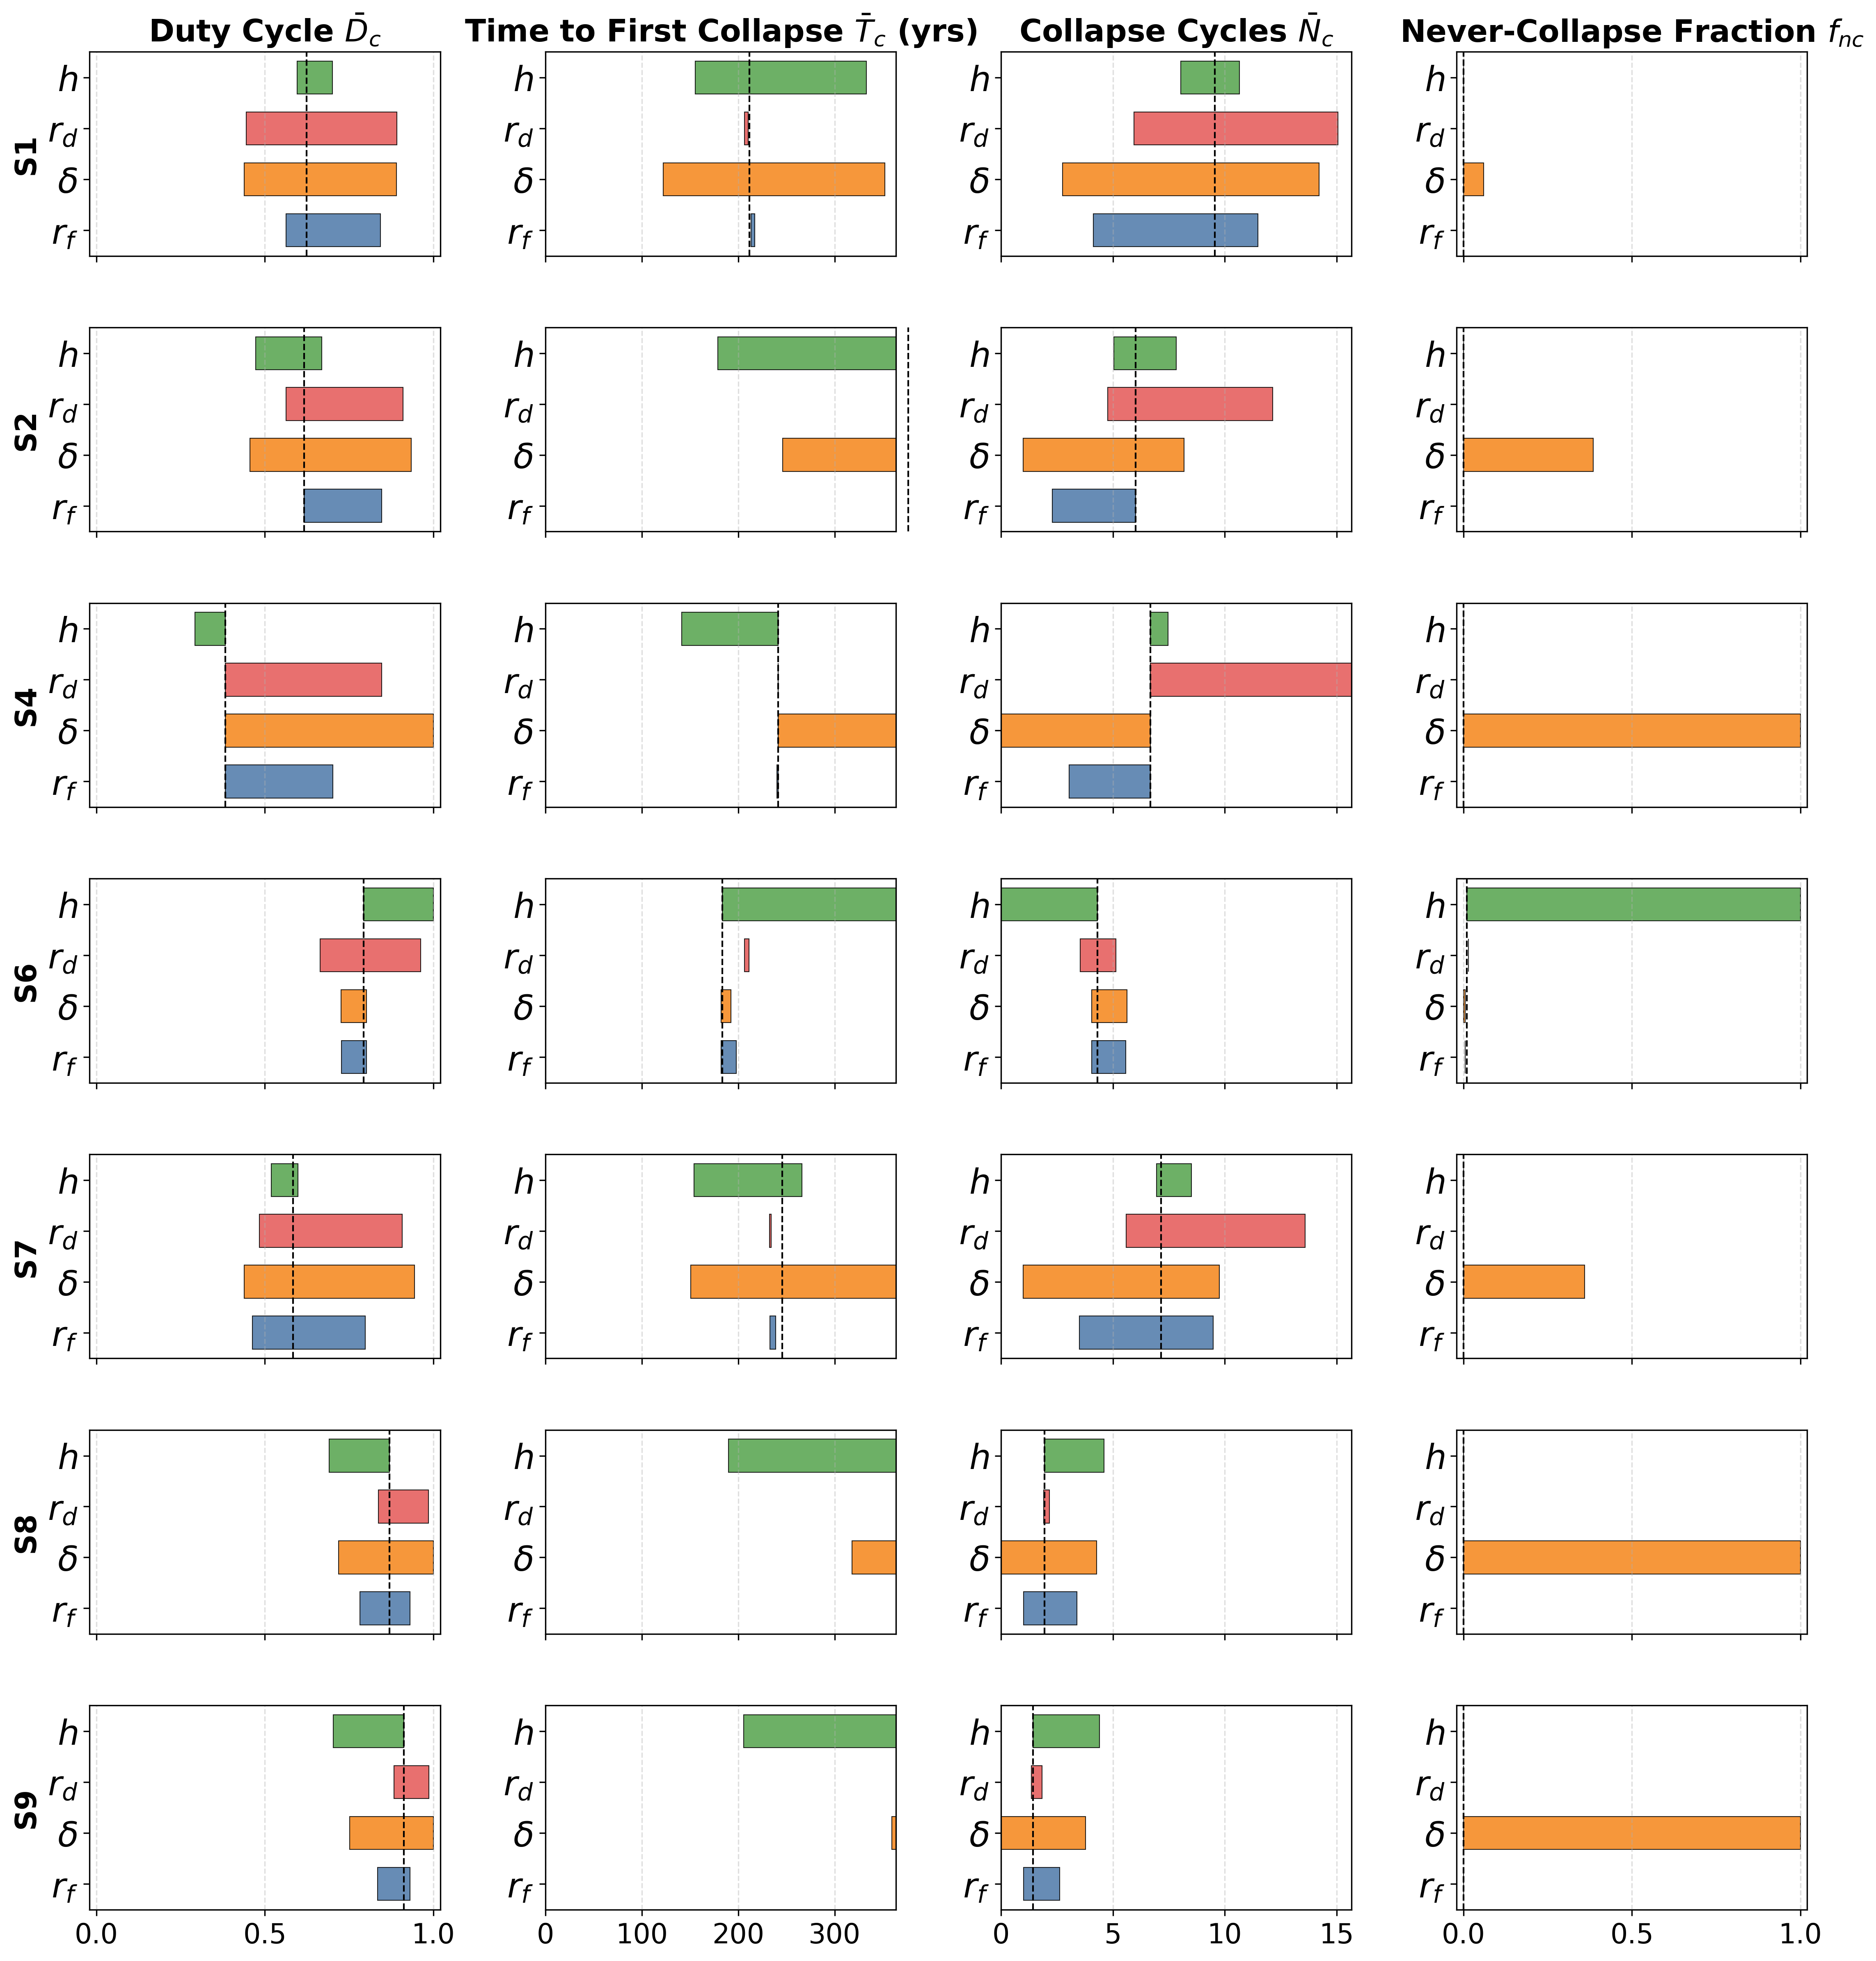
\includegraphics[width=\textwidth,height=0.78\textheight,keepaspectratio]{../figures/sensitivity_analysis_all_scenarios.png}
\caption{Sensitivity analysis for all collapse-prone scenarios. Each row shows one scenario; columns show $\bar{D}_c$, $\bar{T}_c$, $\bar{N}_c$, and $f_{nc}$. Bars span the outcome range when each parameter ($r_f$, $\delta$, $r_d$, $h$) is swept from low to high bound; dashed lines mark baseline values. The parameter $c_f$ is omitted (negligible effect). Note that $h$ dominates in S6 where exogenous risk drives collapse, whereas $r_f$ and $\delta$ are the most impactful levers in resource-limited regimes.}
\label{fig:sensitivity-all}
\end{figure*}

\begin{figure*}[htbp]
\centering
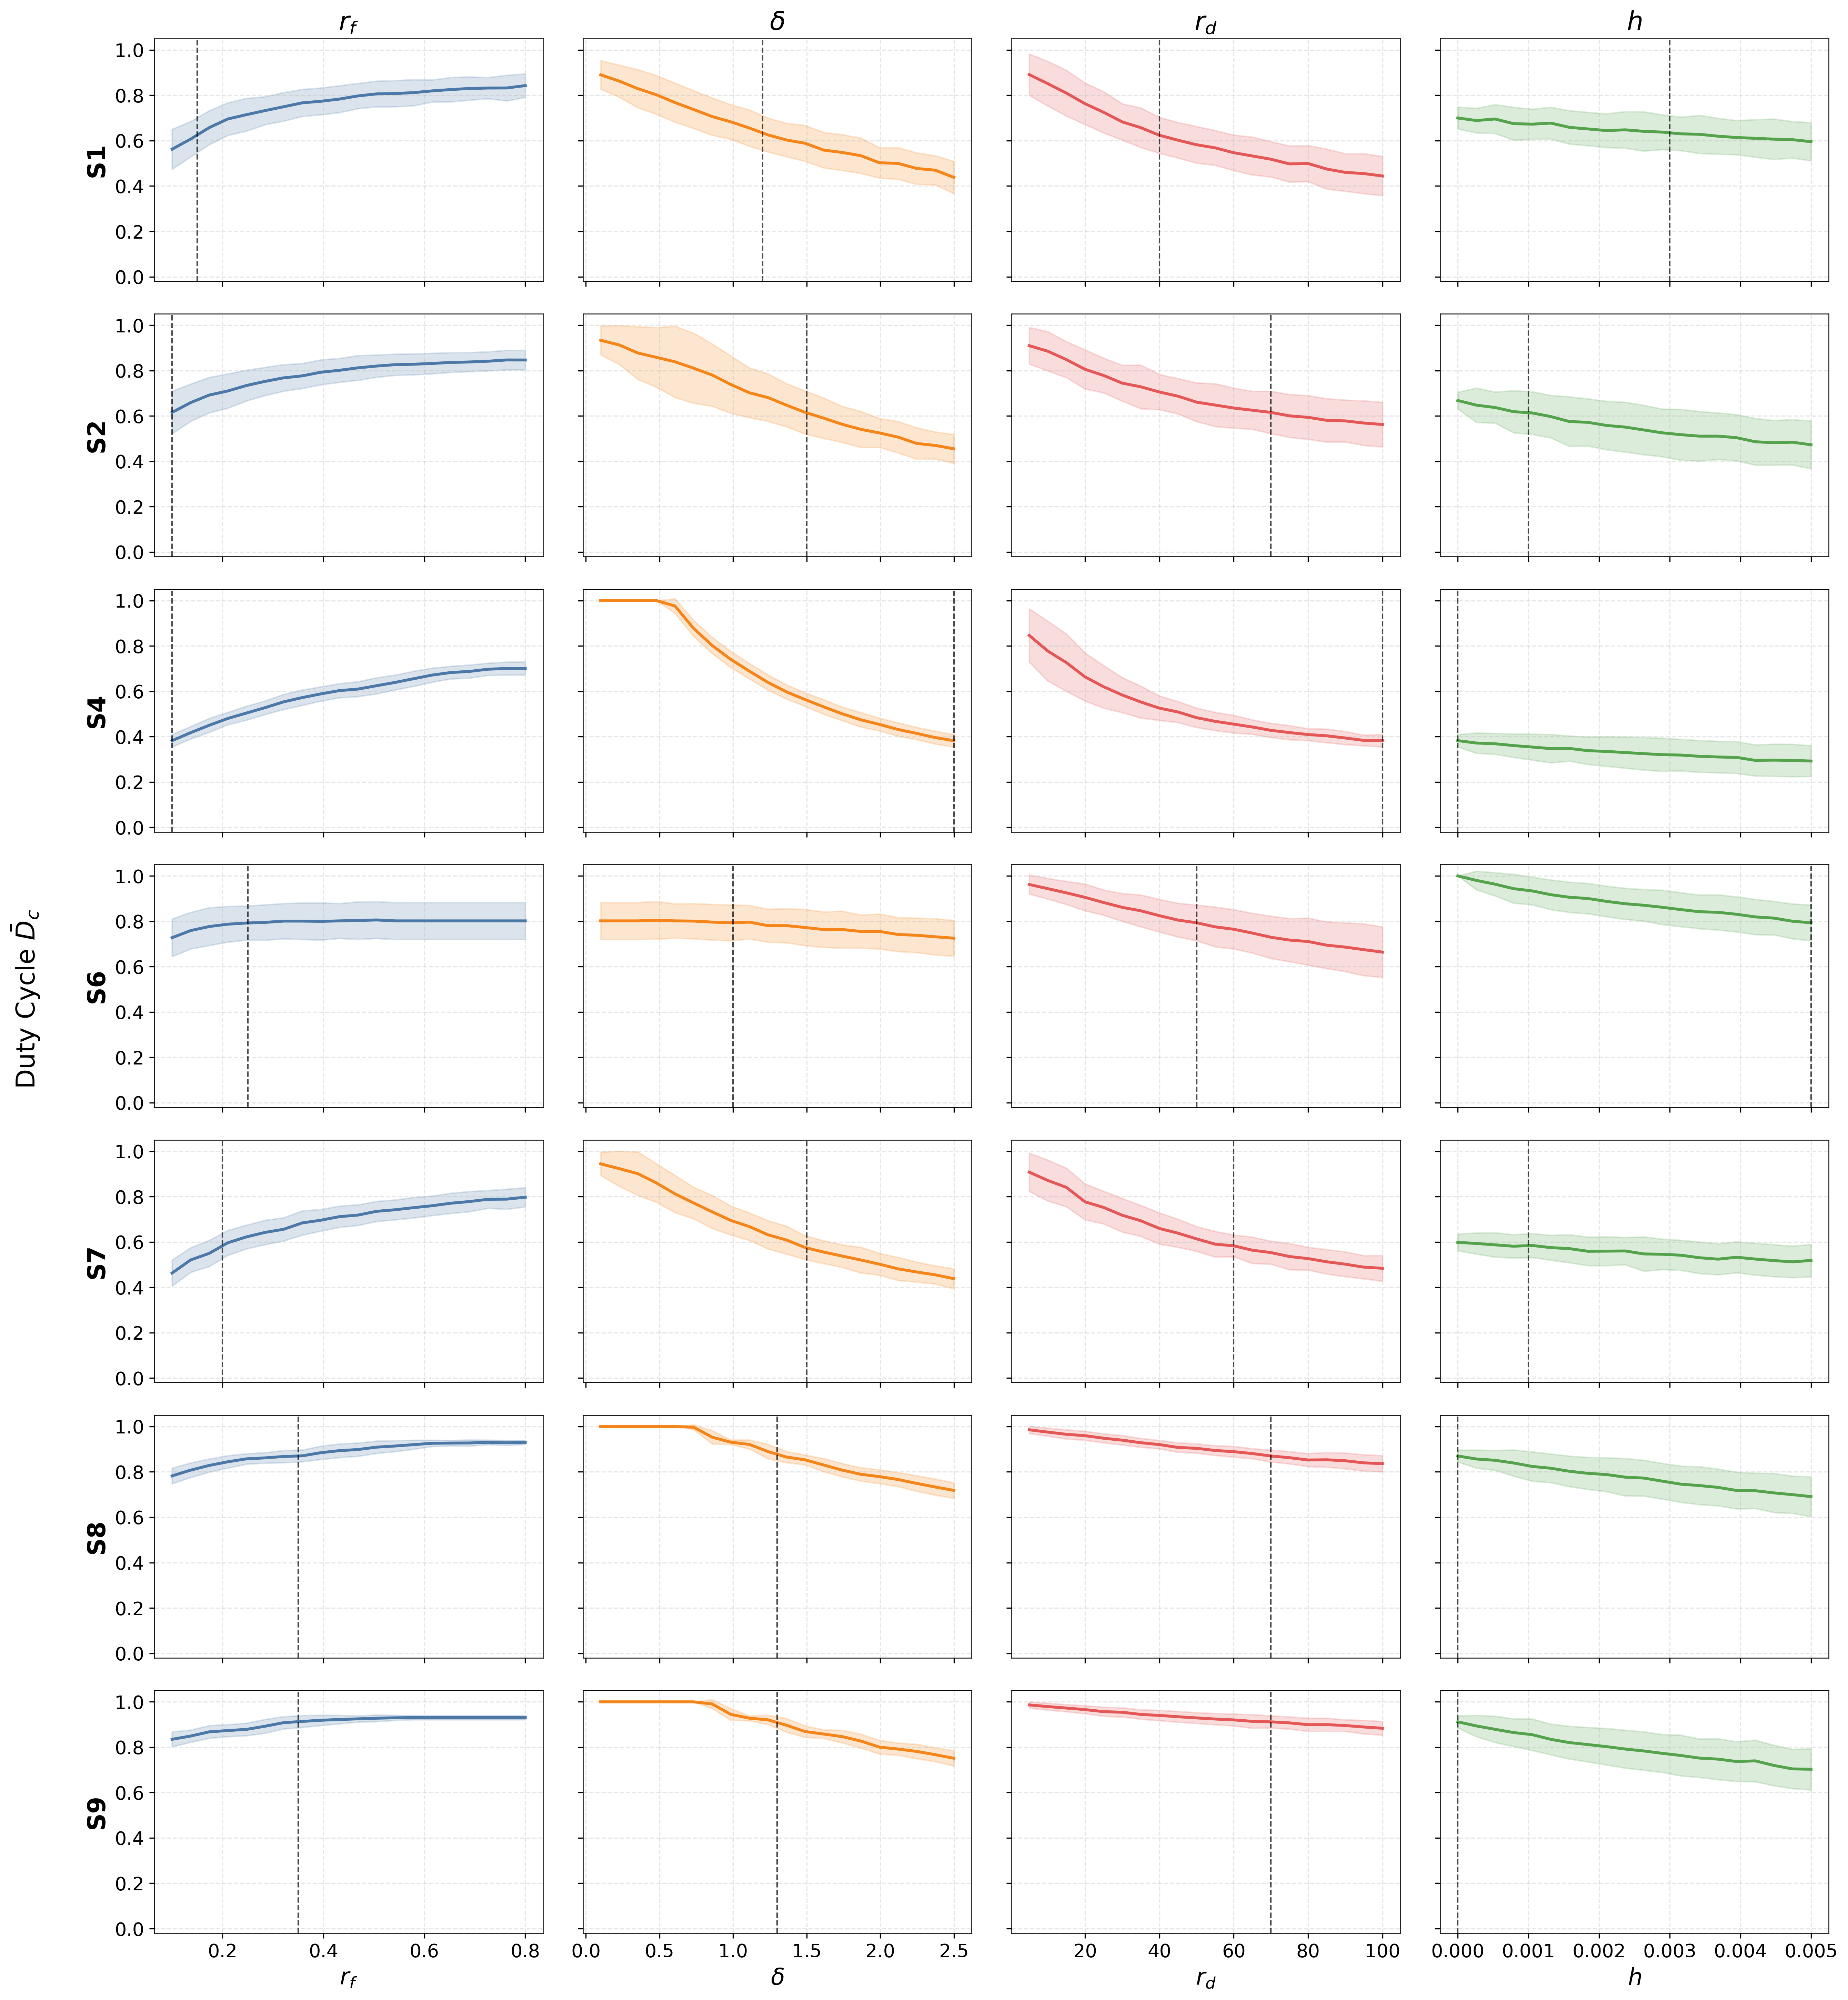
\includegraphics[width=\textwidth,height=0.78\textheight,keepaspectratio]{../figures/sensitivity_response_curves.png}
\caption{Duty cycle $\bar{D}_c$ as a continuous function of each human-controllable parameter for all collapse-prone scenarios (mean $\pm 1\sigma$ over 200 replicates). Each row shows one scenario; columns correspond to the four swept parameters. Dashed lines mark scenario-specific baseline values. The parameter $c_f$ is excluded (negligible effect).}
\label{fig:response-curves}
\end{figure*}